\subsubsection{比较四种方法的清除耗时与计算效率}\label{sec:q3-9}

\Needspace{62mm}
\begin{center}
\begin{minipage}{\linewidth}
\centering\small
\captionof{table}{首版四方法在256个随机场景上的统一比较}
\label{tab:q3-comparison}
\vspace{4pt}
\begin{tabular}{@{}
  >{\raggedright\arraybackslash}p{(\linewidth - 10\tabcolsep) * \real{0.2529}}
  >{\raggedleft\arraybackslash}p{(\linewidth - 10\tabcolsep) * \real{0.1264}}
  >{\raggedleft\arraybackslash}p{(\linewidth - 10\tabcolsep) * \real{0.1264}}
  >{\raggedleft\arraybackslash}p{(\linewidth - 10\tabcolsep) * \real{0.1034}}
  >{\centering\arraybackslash}p{(\linewidth - 10\tabcolsep) * \real{0.2529}}
  >{\centering\arraybackslash}p{(\linewidth - 10\tabcolsep) * \real{0.1379}}@{}}
\toprule
\begin{minipage}[b]{\linewidth}\raggedright
方法
\end{minipage} & \begin{minipage}[b]{\linewidth}\raggedleft
均时 / s
\end{minipage} & \begin{minipage}[b]{\linewidth}\raggedleft
P95 / s
\end{minipage} & \begin{minipage}[b]{\linewidth}\raggedleft
节省
\end{minipage} & \begin{minipage}[b]{\linewidth}\centering
节省95\%区间 / s
\end{minipage} & \begin{minipage}[b]{\linewidth}\centering
全清
\end{minipage} \\
\midrule
前瞻基线 & 3361.66 & 3843.91 & --- & --- & 256/256 \\
状态搜索 & 3081.41 & 3520.79 & 8.34\% & {[}259.47, 301.17{]} & 256/256 \\
PPO & 3149.79 & 3624.61 & 6.30\% & {[}187.04, 237.12{]} & 256/256 \\
几何法 & 3214.96 & 3604.87 & 4.36\% & {[}125.79, 167.35{]} & 256/256 \\
\bottomrule
\end{tabular}
\end{minipage}
\end{center}

四种方法共 1136 次评估均完整清除、正常结束，失败清除次数为零。
状态搜索的随机集均时最低，比基线平均节省 280.25 s；
PPO 与几何法也有正向平均改善。
几何法未达到预先设置的平均节省 5\% 门槛，但这不等于没有改善。
28个压力场景中，基线、状态搜索、PPO和几何法均时分别为3627.40、3046.34、3164.37和3254.15 s，均为28/28局全清。
状态搜索相对基线为 28 胜 0 负，PPO 为 25 胜 3 负，几何法为 26 胜 2 负；
这些针对固定困难类型的结果不与随机集混合计算总体均值。

费用分解显示，状态搜索相较基线少用移动时间 212.68 s、测量时间 62.38 s、换频时间 5.18 s；
光学检查与移除费用相同。
由此可见，联合安排覆盖与清除任务的主要收益体现在行程缩短，同时减少了部分测量。
该分解说明实际费用来源，不能把全部路线收益归因于某一个模块。
首版状态搜索、PPO 和几何法相对基线的最坏单局仍分别慢 125.08、365.45 和 267.73 s，平均改善不代表逐局不劣。

\begin{figure}[!htbp]
\centering
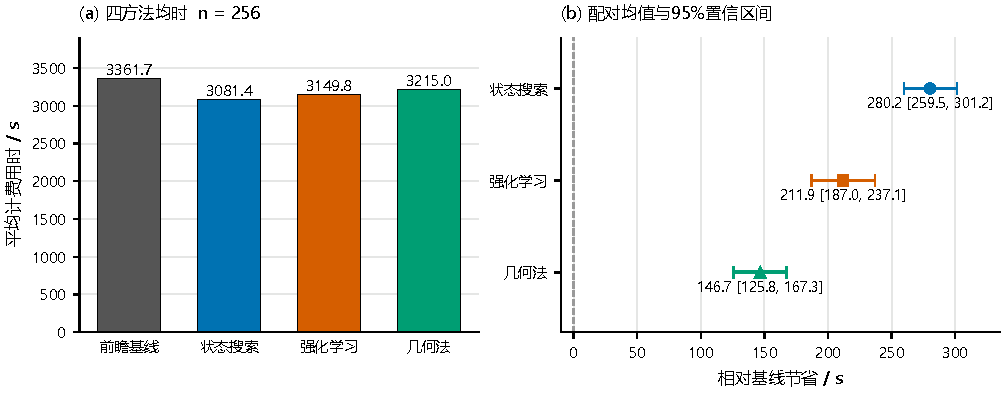
\includegraphics[width=\linewidth,height=\textheight,keepaspectratio,alt={首版四方法在同一256随机场景上的均时与配对节省。右图为相对前瞻基线的95\%配对bootstrap区间，不能当作左图各均时的区间。}]{figures/fig03_comparison.pdf}
\caption{首版四方法在同一256随机场景上的均时与配对节省。右图为相对前瞻基线的95\%配对bootstrap区间，不能当作左图各均时的区间。}
\label{fig:q23-3}
\end{figure}

\begin{figure}[!htbp]
\centering
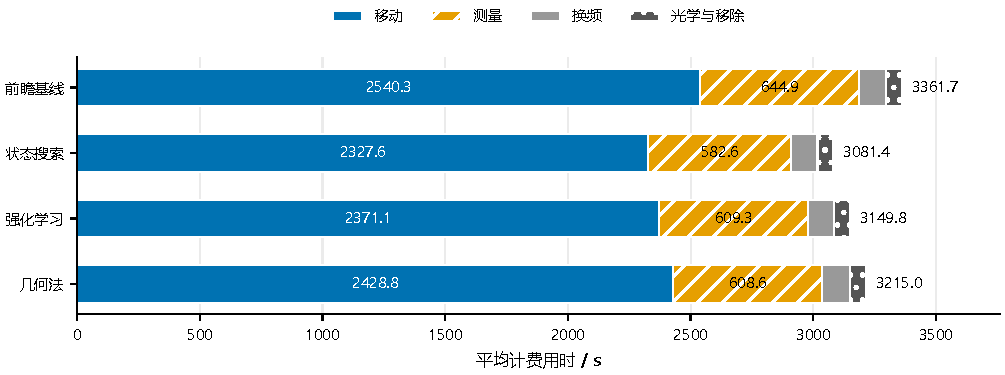
\includegraphics[width=\linewidth,height=\textheight,keepaspectratio,alt={首版随机集的平均费用分解。分项之和等于整局计费用时；移动是主要成本，但扫描与换频的节省同样影响总结果。}]{figures/fig04_costs.pdf}
\caption{首版随机集的平均费用分解。分项之和等于整局计费用时；移动是主要成本，但扫描与换频的节省同样影响总结果。}
\label{fig:q23-4}
\end{figure}

算法计算速度与机器人执行效率需要区分。
在同一 Linux CPU 上，四种方案以单线程串行运行已用开发场景，预热后重复两遍，共计每方法 32 局；
平均实际计算时间依次为 5.845、0.592、0.170 和 2.098 s/局。
PPO 部署计算最快，状态搜索的机器人虚拟耗时最低；
该计时包含策略与仿真接口，不等同于纯网络推理延迟，也不是新增的泛化测试。

\subsubsection{通过消融实验分析各项策略的作用}\label{sec:q3-10}

首先检验可证明无信号的测量能否直接省略。
在长轴分位探点策略上，仅增加``候选源区域到待测点的最小距离超过最大接收半径''的删测条件，冻结后 64 局平均从 3132.57~s 降至 3119.32 s，节省 13.25 s，95\% 区间为 {[}9.75,16.97{]} s。
移动轨迹保持相同，收益来自检测与换频；
未知频道仍执行真实覆盖扫描。
这一结果将几何证书的作用与路线调整较清楚地区分开来。

其次，在上述策略基础上仅允许未来覆盖站移到仍满足全场覆盖的位置。
另 64 局确认的均时由 3100.20 s 降至 3073.60 s，平均节省 26.59 s，区间为 {[}3.11,53.17{]} s。
44 局改善、20 局退化，最坏慢 215.29 s，表明冻结任务上的路线缩短可能被后续发现顺序与定位路径变化抵消。
因而，覆盖移站有小幅平均收益证据，但尚不支持所有场景不退化的保证。

后续将真实负反馈与当前候选区域组合，构造更强的相对无信号证书，并加入发现第 16 个源后停止查询未发现频道的规则。
在新的 256 局最终随机集上，原 v1 均时为 3122.26 s；
仅相对证书、仅数量上限和二者组合分别节省 13.11、1.72 和 14.83 s，对应区间为 {[}11.52,14.74{]}、{[}1.13,2.39{]} 和 {[}13.03,16.70{]} s。
组合的改善为 0.475\%，190 胜、66 平、0 负；
另 28 局压力集也全部完成。
组合在随机集共省 631 次查询，实际节省 3796 s，其中检测 3155 s、换频 641 s，移动费用逐局一致。
四局因当前频道改变出现站内重排，故不能笼统声称全部轨迹仅做删除。
这批结果支持小幅、可解释的改进，不能与前述不同场景上的均值相减或机械叠加各模块收益。

\begin{figure}[!htbp]
\centering
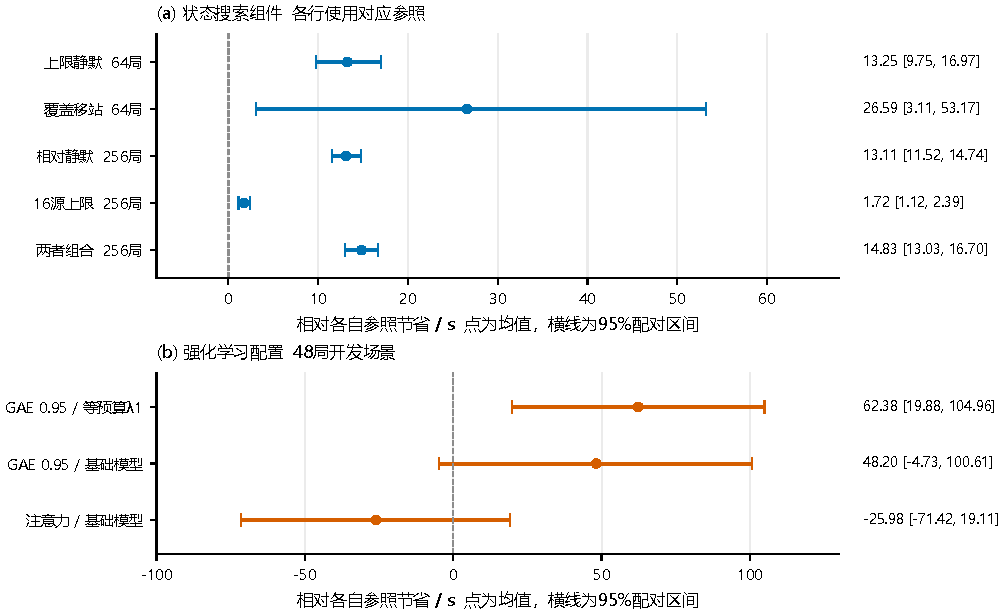
\includegraphics[width=\linewidth,height=\textheight,keepaspectratio,alt={核心组件及训练配置的消融结果。正值表示节省，各行以各自冻结参照计算；上部的64局和256局来自不同实验批次，下部为48局开发结果。不同批次收益不作相加。}]{figures/fig05_ablations.pdf}
\caption{核心组件及训练配置的消融结果。正值表示节省，各行以各自冻结参照计算；上部的64局和256局来自不同实验批次，下部为48局开发结果。不同批次收益不作相加。}
\label{fig:q23-5}
\end{figure}

